\section{Preventivo}

Per facilitare la lettura delle tabelle, vengono utilizzate le seguenti sigle per identificare i ruoli:

\begin{itemize}
\item \textbf{RE:} \respProg;
\item \textbf{AM:} \ammProg;
\item \textbf{AN:} \analProg;
\item \textbf{PT:} \progetProg;
\item \textbf{PR:} \programProg;
\item \textbf{VE:} \verifProg.
\end{itemize}

\subsection{Fase di analisi}
\subsubsection{Prospetto orario}
In questa fase, la distribuzione oraria dei componenti del gruppo è la seguente:

{

\rowcolors{2}{azzurro2}{azzurro3}

\centering
\renewcommand{\arraystretch}{1.8}
\begin{longtable}{C{4cm} C{1cm} C{1cm} C{1cm} C{1cm} C{1cm} C{1cm} C{2cm}}

\rowcolor{azzurro1}
\textbf{Nominativo} &
\textbf{RE}&
\textbf{AM}&
\textbf{AN}&
\textbf{PT}&
\textbf{PR}&
\textbf{VE}&
\textbf{Ore totali}\\
\endhead

\MB & 15 & 0 & 12 & 0 & 0 & 8 & 35 \\
\VAS & 0 & 18 & 5 & 0 & 0 & 12 & 35 \\
\FD & 10 & 8 & 5 & 0 & 0 & 12 & 35 \\
\NM & 0 & 20 & 5 & 0 & 0 & 10 & 35 \\
\SB & 0 & 18 & 7 & 0 & 0 & 10 & 35 \\
\GB & 0 & 0 & 22 & 0 & 0 & 13 & 35 \\
\MDI & 0 & 0 & 24 & 0 & 0 & 11 & 35 \\
\textbf{Ore Totali} & 25 & 64 & 80 & 0 & 0 & 76 & 245 \\

\rowcolor{white}
\caption{Distribuzione oraria nel periodo di analisi}\\

\end{longtable}
}
\newpage
Il seguente istogramma riassume i dati ottenuti:

\begin{figure}[H]
\centering
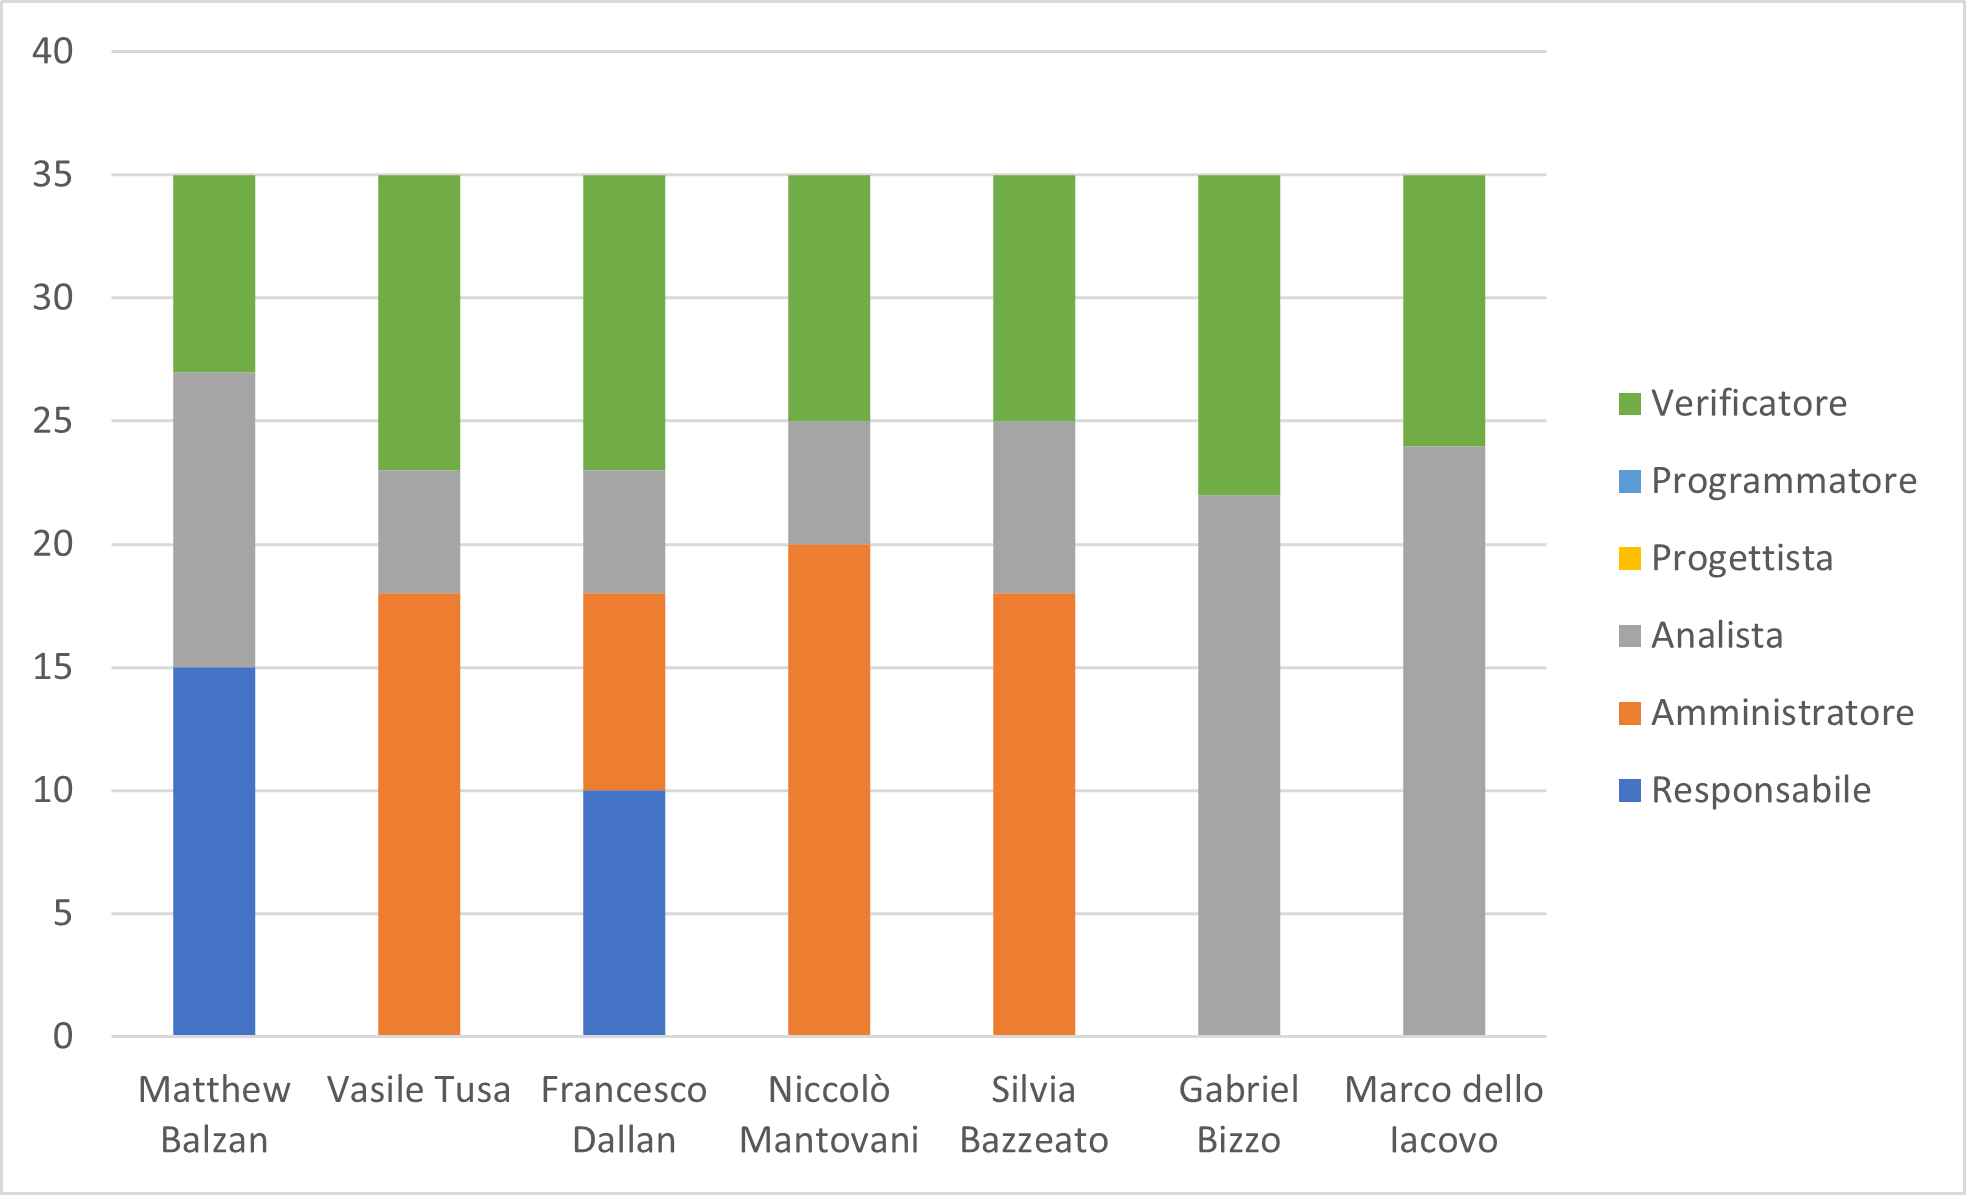
\includegraphics[scale=0.90]{res/Preventivo/Img/istogramma_analisi}\\
\caption{Istogramma della ripartizione dei ruoli nel periodo di analisi}
\end{figure}


\subsubsection{Prospetto economico}

In questa fase, il costo per ogni ruolo è il seguente:

{

\rowcolors{2}{azzurro2}{azzurro3}

\centering
\renewcommand{\arraystretch}{1.8}
\begin{longtable}{C{3cm} C{1cm} C{2cm} }

\rowcolor{azzurro1}
\textbf{Ruolo} &
\textbf{Ore}&
\textbf{Costo}\\
\endhead

\textit{Responsabile} & 25 & 750\euro{} \\
\ammProg & 64 & 1280\euro{} \\
\analProg & 80 & 2000\euro{} \\
\progetProg & 0 & 0\euro{} \\
\programProg & 0 & 0\euro{} \\
\verifProg & 76 & 1140\euro{} \\
\textbf{Totale} & 245 & 5170\euro{} \\

\rowcolor{white}
\caption{Prospetto dei costi per ruolo nel periodo di analisi}\\

\end{longtable}
}
\newpage
Il seguente areogramma riassume i dati ottenuti:

\begin{figure}[H]
\centering
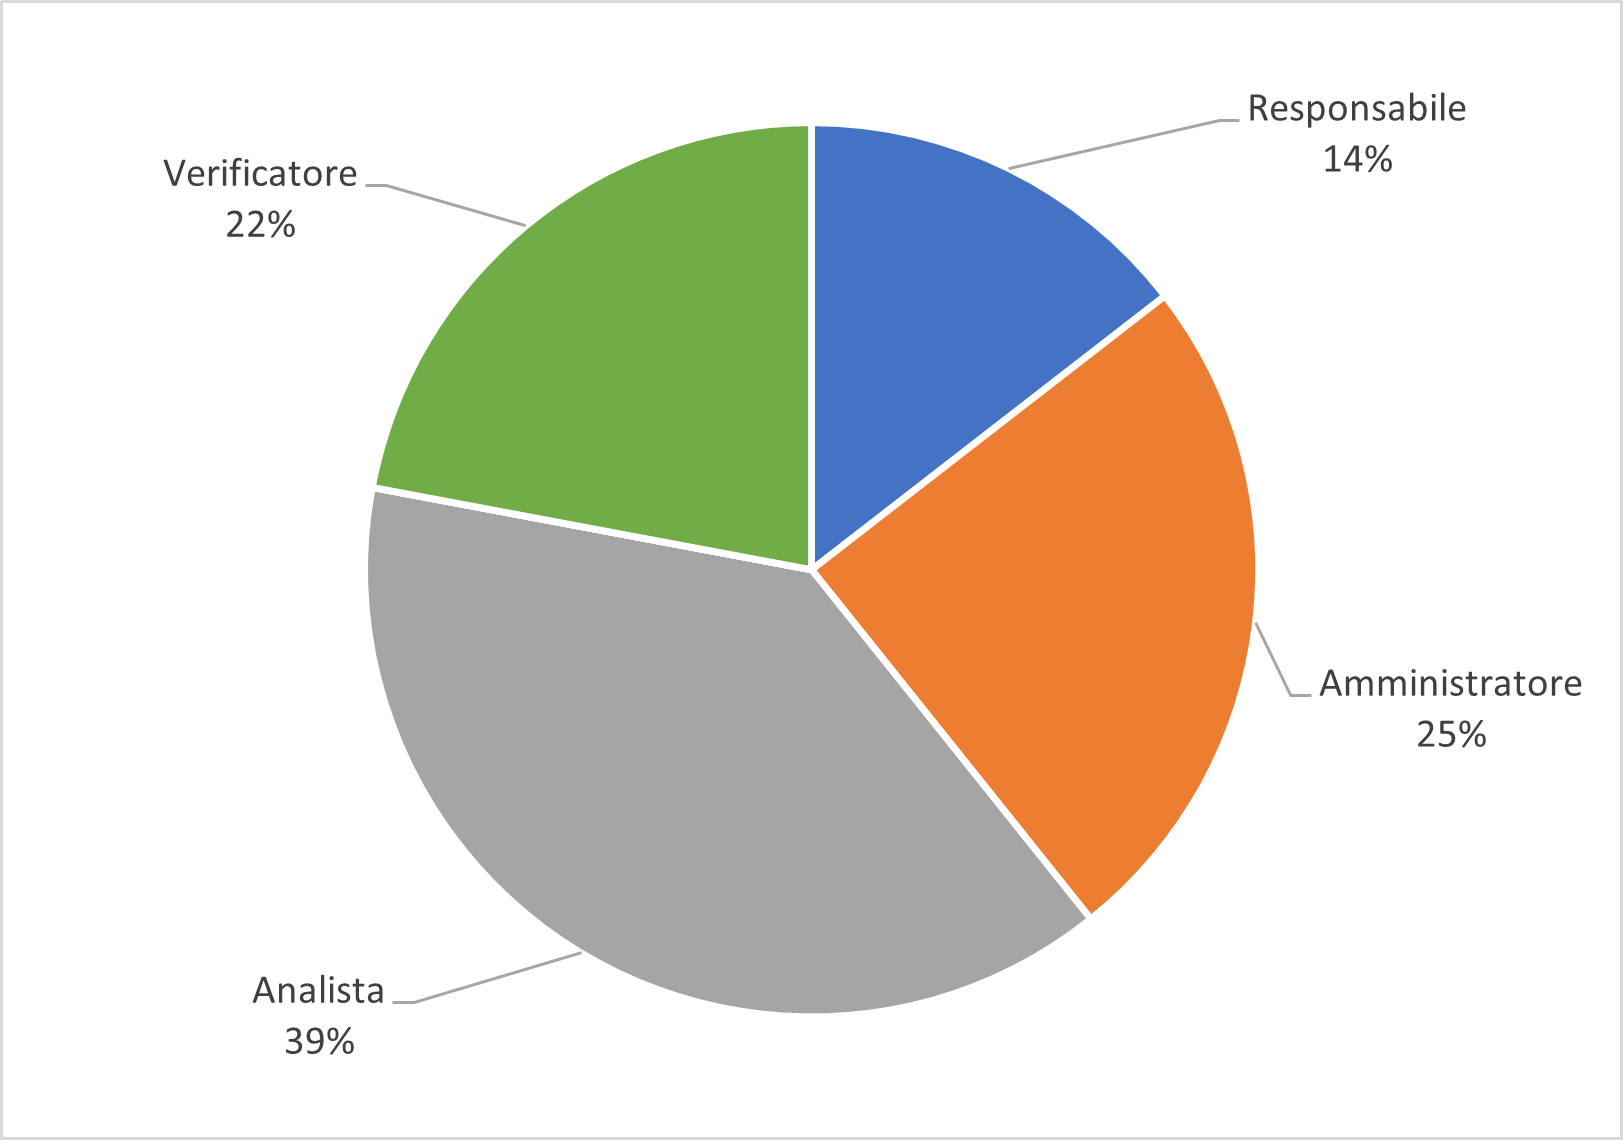
\includegraphics[scale=0.90]{res/Preventivo/Img/areogramma_analisi}\\
\caption{Areogramma della distribuzione economica nel periodo di analisi}
\end{figure}



\subsubsection{Progettazione}
\myparagraph{Scopo}
L'attività di progettazione precede la codifica e ha il compito di individuare i requisiti software richiesti (analizzando l' \AdRv{2.0.0}) per far si che il prodotto finale soddisfi tutti gli stakeholder\ped{G}. Per far ciò lo sviluppo del prodotto deve essere:
\begin{itemize}
\item \textbf{Efficiente}: prodotto in economia, minimizzando le risorse utilizzate;
\item \textbf{Efficace}: deve garantire la qualità del prodotto perseguendo la correttezza per costruzione;
\item \textbf{Organizzato}: i compiti devono essere suddivisi tra i vari membri del gruppo in modo da ridurre la complessità del problema.
\end{itemize}

\myparagraph{Aspettative}
Il gruppo \Omicron{} intende, tramite l'attività di progettazione, fissare l'architettura del prodotto prima di passare alla sua realizzazione. 

\myparagraph{Descrizione}
Le parti fondamentali del processo di progettazione sono due:
\begin{itemize}
\item \textbf{Technology baseline}: è redatta dal progettista e contiene:
\begin{itemize}
\item specifiche della progettazione ad alto livello del prodotto e delle sue componenti;
\item elenco dei diagrammi UML\ped{G} che saranno utilizzati per la realizzazione dell'architettura e dei test di verifica.
\end{itemize}
\item \textbf{Product baseline}: è redatta dal progettista e ha il compito di:
\begin{itemize}
\item integrare ciò che è riportato nella Technology baseline;
\item definire i test di verifica.
\end{itemize}
\end{itemize} 

\myparagraph{Technology baseline}
Le \textbf{Technology baselines} includono:
\begin{itemize}
\item \textbf{Diagrammi UML\ped{G}}:
\begin{itemize}
\item \textbf{diagrammi delle classi}: descrivono il tipo degli oggetti che compongono il sistema e le relazioni statiche esistenti tra loro;
\item \textbf{diagrammi dei package}: documentano le dipendenze fra le classi;
\item \textbf{diagrammi di attività}: descrivono le azioni di un processo;
\item \textbf{diagrammi di sequenza}: descrive uno scenario, ovvero una serie di azioni in cui tutte le scelte sono già effettuate.
\end{itemize}
\item \textbf{Design Pattern\ped{G}}: soluzioni progettuali generali ad un problema ricorrente. Devono essere descritti e rappresentati con un diagramma che ne espone significato e struttura;
\item \textbf{Tecnologie utilizzate}: descrizione delle tecnologie usate. Ne devono essere descritti l'utilizzo, i vantaggi e gli svantaggi;
\item \textbf{Tracciamento delle componenti}: i requisiti vengono soddisfatti da alcune componenti, di cui vi è necessità di tener traccia;
\item \textbf{Test di integrazione}: test il cui scopo è assicurarsi il corretto funzionamento del progetto una volta che sono state unite le sue componenti.
\end{itemize}

\myparagraph{Product baseline}
Le \textbf{Product baselines} includono:
\begin{itemize}
\item \textbf{definizione delle classi}: di ogni classe è necessario che si possano comprendere in modo esaustivo lo scopo e le funzionalità, evitando ridondanze;
\item \textbf{tracciamento delle classi}: ogni requisito deve avere una classe che lo soddisfi; 
\item \textbf{test di unità}: test il quale scopo è assicurarsi il corretto funzionamento delle singole componenti del progetto.
\end{itemize}
\subsubsection{Codifica}
\myparagraph{Scopo}
L'attività di codifica ha lo scopo di normare l'effettiva realizzazione del prodotto software partendo dall'architettura realizzata durante la fase di progettazione. È compito del programmatore assicurarsi il corretto svolgimento di questa attività.

\myparagraph{Aspettative}
L'obiettivo del gruppo \Omicron{} è quello di creare, tramite l'attività di codifica, un prodotto software che sia in grado di soddisfare i requisiti prefissati con il proponente assicurandosi, usando delle norme e delle convenzioni, di:
\begin{itemize}
\item generare codice leggibile ed uniforme;
\item agevolare le fasi di manutenzione, verifica e validazione;
\item mantenere un prodotto di ottima qualità. 
\end{itemize}

\myparagraph{Descrizione}
Il codice scritto dovrà essere di qualità, rispettando e perseguendo gli obiettivi di qualità definiti nel \PdQv.

\myparagraph{Stile di codifica}
Il codice generato da ogni membro deve rispettare le seguenti norme:
\begin{itemize}
\item \textbf{indentazione}: Ogni blocco innestato deve essere indentato usando 2 spazi per ogni livello di indentazione;
\item \textbf{parentesizzazione}: le parentesi di delimitazione dei costrutti devono essere inserite in linea e non al di sotto di essi;
\item \textbf{scrittura dei metodi}: è preferibile l'uso di metodi brevi (con poche righe di codice);
\item \textbf{univocità dei nomi}: il nome di classi, metodi, variabili deve essere univoco e autoesplicativo;
\item \textbf{struttura dei nomi}: I nomi sono strutturati nel seguente modo:
\begin{itemize}
\item \textit{metodi, variabili e costanti}: sono scritti con la prima lettera minuscola. Se il nome è composto da più parole quelle successive iniziano con la lettera maiuscola (camel Case);
\item \textit{classi}: sono scritti con la prima lettera maiuscola. Se il nome è composto da più parole quelle successive iniziano con la lettera maiuscola (Pascal Case).
\end{itemize} 
\item \textbf{lingua}: il codice e i commenti saranno scritti in lingua italiana.
\end{itemize}

\myparagraph{Ricorsione}
L'uso della ricorsione va evitato se non in casi dove risulta essere strettamente necessaria.

\subsection{Validazione e collaudo}
\textit{\textbf{Periodo}: dal 2021-04-23 al 2021-05-26}

L'inizio di questa fase coincide con data della Revisione di Qualifica e si conclude con la scadenza della Revisione di Accettazione.

\subsubsection{Attività}

\begin{itemize}
\item \textbf{Incremento e verifica documenti}: vengono realizzati gli incrementi necessari ai documenti. I documenti in questione sono:
\begin{itemize}
\item \NdP{};
\item \AdR{};
\item \PdQ{};
\item \PdP{};
\item Glossario;
\item \MU{};
\item \MM{}.
\end{itemize}
\item \textbf{Validazione e collaudo}: viene completato il prodotto e i documenti in base a requisiti mancanti, indicazioni del proponente o analisi interne. Vengono inoltre eseguiti tutti i test per validare e collaudare il prodotto finale.
\item \textbf{Consolidamento}: viene realizzata la presentazione da esporre in sede di Revisione di Accettazione.
\end{itemize}

\subsubsection{Incremento 11}
\myparagraph{Consuntivo}

{

\rowcolors{2}{azzurro2}{azzurro3}

\centering
\renewcommand{\arraystretch}{1.8}
\begin{longtable}{C{4cm} C{1.5cm} C{4cm} }

\rowcolor{azzurro1}
\textbf{Ruolo} &
\textbf{Ore}&
\textbf{Costo}\\
\endhead

\textit{Responsabile} & 5 (+0) & 150 (+0\euro{}) \\
\ammProg & 6 (+0) & 120\euro{} (+0\euro{}) \\
\analProg & 0 (+0) & 0\euro{} (+0\euro{}) \\
\progetProg & 11 (+0) & 242\euro{} (+0\euro{}) \\
\programProg & 13 (+2) & 195\euro{} (+30\euro{}) \\
\verifProg & 16 (+0) & 240\euro{} (+0\euro{})\\
\textbf{Totale Preventivo} & \textbf{51} & \textbf{947\euro{}} \\
\textbf{Totale Consuntivo} & \textbf{53} & \textbf{977\euro{}} \\
\textbf{Differenza} & \textbf{+2} & \textbf{+30\euro{}} \\


\rowcolor{white}
\caption{Consuntivo di periodo dell'incremento 11}\\

\end{longtable}
}

\myparagraph{Considerazioni}
In questo incremento sono state implementate le ultime funzionalità previste per il nostro prodotto, che ha però portato ad un ritardo e un impegno maggiore di quanto previsto. In particolare sono state trovate alcune problematiche nello sviluppo delle pagine statiche incrementali e nell'autenticazione delle API\ped{G}, ma che sono state risolte tramite ricerche\\
Nonostante ciò, la produzione degli incrementi documentali è risultata come prevista inizialmente.
Dato il ritardo di completamento di questo incremento ed una discussione sugli impegni individuali dei componenti del gruppo durante la fase corrente, è stata effettuata una ripianificazione temporale degli incrementi successivi, lasciando comunque invariato l'impegno orario. Rimangono invariati gli obiettivi dei successivi incrementi.



\myparagraph{Preventivo a finire}
Il bilancio risulta leggermente negativo rispetto al preventivo dell'incremento, con una perdita di 30\euro{}. Esso viene però sanato dal risparmio precedente di 36\euro{}, risultando in un risparmio totale di 6\euro{}.\\ 
Date le considerazioni precedenti e con il bilancio totale ancora in positivo, riteniamo di essere in linea con il preventivo e non prevediamo cambiamenti drastici di esso.


\subsubsection{Incremento 12}
\textit{\textbf{Periodo}: dal 2021-04-30 al 2021-05-08}

\myparagraph{Obiettivi}
Gli obiettivi definiti per questo incremento sono i seguenti:
\begin{itemize}
\item implementazione test mancanti;
\item esecuzione test di sistema;
\item incremento della documentazione, con eventuale correzione in base a segnalazione dei committenti.
\end{itemize}

\myparagraph{Attività}
Per raggiungere gli obiettivi, vengono svolte le seguenti attività:
\begin{itemize}
\item \textbf{codifica}: 
\begin{itemize}
\item implementazione ulteriori test mancanti;
\item correzione di eventuali bug.
\end{itemize} 

\item \textbf{verifiche del prodotto}: esecuzione di test di sistema per l'intero prodotto;

\item \textbf{ampliamento documentazione e verifiche}:
\begin{itemize}
\item eventuali correzioni dei documenti segnalati dai committenti;
\item incremento del \MUv{0.1.0} in base ai test effettuati;
\item incremento del \MMv{0.1.0} in base ai test effettuati;
\item incremento del \Glossariov{3.0.0};
\item rilevazione e registrazione di metriche, esiti di verifica e obiettivi di qualità;
\item aggiornamento dei rischi rilevati;
\item calcolo e registrazione del consuntivo di periodo.
\end{itemize}

\end{itemize}
\myparagraph{Diagramma di Gantt}
\begin{figure}[H]
\centering

\centerline{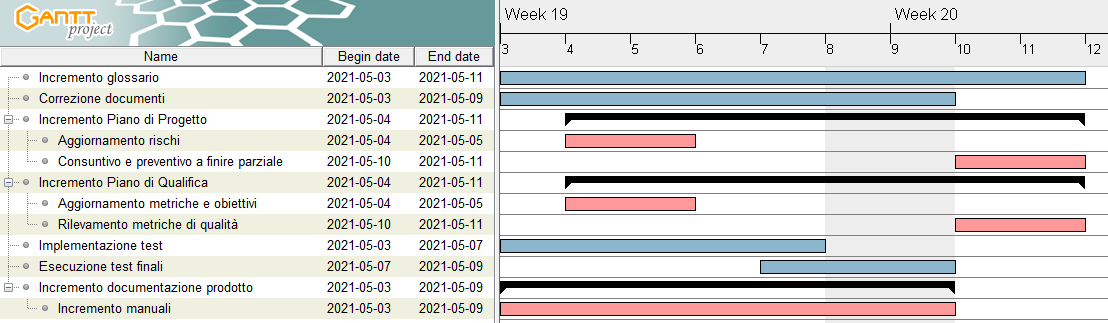
\includegraphics[scale=0.6]{res/Pianificazione/Fasi/VerificaIncrementi/ganttIncremento12}}
\caption{Diagramma di Gantt per l'incremento 12}
\end{figure}
\subsubsection{Incremento 13}
\textit{\textbf{Periodo}: dal 2021-05-09 al 2021-04-17}

\myparagraph{Obiettivi}
Gli obiettivi definiti per questo incremento sono i seguenti:
\begin{itemize}

\item preparazione alla presentazione della Revisione di Accettazione;
\item preparazione al collaudo finale con il proponente;
\item incremento della documentazione.
\end{itemize}

\myparagraph{Attività}
Per raggiungere gli obiettivi, vengono svolte le seguenti attività:
\begin{itemize}
\item \textbf{presentazione Revisione di Accettazione}: creazione e preparazione della presentazione con il \VT{};
\item \textbf{collaudo}: controlli e verifiche ultime al prodotto e ai documenti per il collaudo finale con il proponente;
\item \textbf{ampliamento documentazione e verifiche}:
\begin{itemize}
\item incremento del \Glossariov{4.0.0};
\item rilevazione e registrazione di metriche, esiti di verifica e obiettivi di qualità;
\item aggiornamento dei rischi rilevati;
\item calcolo e registrazione del consuntivo di periodo.
\end{itemize}

\end{itemize}
\myparagraph{Diagramma di Gantt}
\begin{figure}[H]
\centering

\centerline{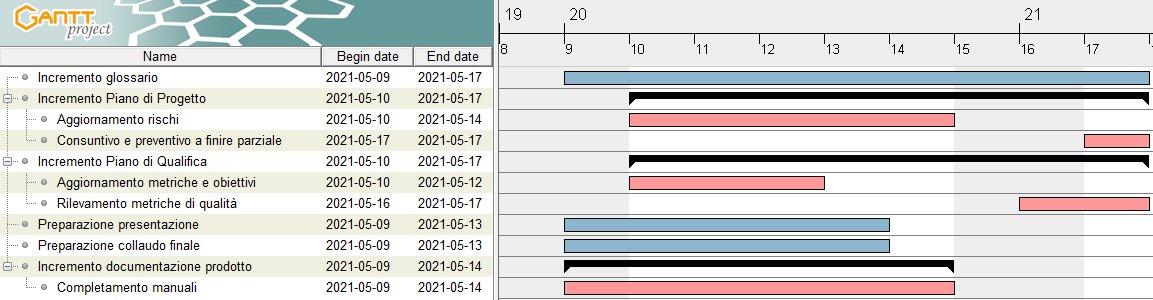
\includegraphics[scale=0.6]{res/Pianificazione/Fasi/VerificaIncrementi/ganttIncremento13}}
\caption{Diagramma di Gantt per l'incremento 13}
\end{figure}
\subsection{Riepilogo}
\subsubsection{Ore totali}
\paragraph{Suddivisione del lavoro}
\paragraph{Prospetto economico}

\subsubsection{Ore rendicontate}
\paragraph{Suddivisione del lavoro}
\paragraph{Prospetto economico}


\subsubsection{Conclusioni}

Il costo totale preventivato per il progetto, considerando solo le ore rendicontate, è 13.154,00\euro{}.

